\chapter{Integracija dva sustava}

Svaka od komponenti sustava implementirana je u zasebnom projektu, sličnosti izvornih kodova su implementirane uz $Turtle$ dok je određivanje autorstva implementirano u projektu nazvanom $Bee$. $Bee$ je dizajniran kao skripta komandne linije kojoj se predaju skup za treniranje i skup za testiranje te koja vraća točnost naučenog klasifikatora. Pošto je $Turtle$ web aplikacija bilo je potrebno nekako spojiti ova dva sustava. To je napravljeno tako da je u $Bee$ napisan mali web server koji nudi nekoliko API endpoint-a za treniranje i predikciju. Te API endpoint-e koristi klijentski kod $Turtle$ te su dvije aplikacije tako integrirane. Razloga za ovakvu integraciju je nekoliko, ali najvažniji je fleksibilnost, pošto sada funkcije $Bee$ možemo koristiti kroz više različitih aplikacija. 

\section{Korisničko sučelje}

U ovom potpoglavlju opisano je korisničko sučelje sustava $Turtle$ kroz nekoliko slika.


\begin{figure}[htb]
	\centering
	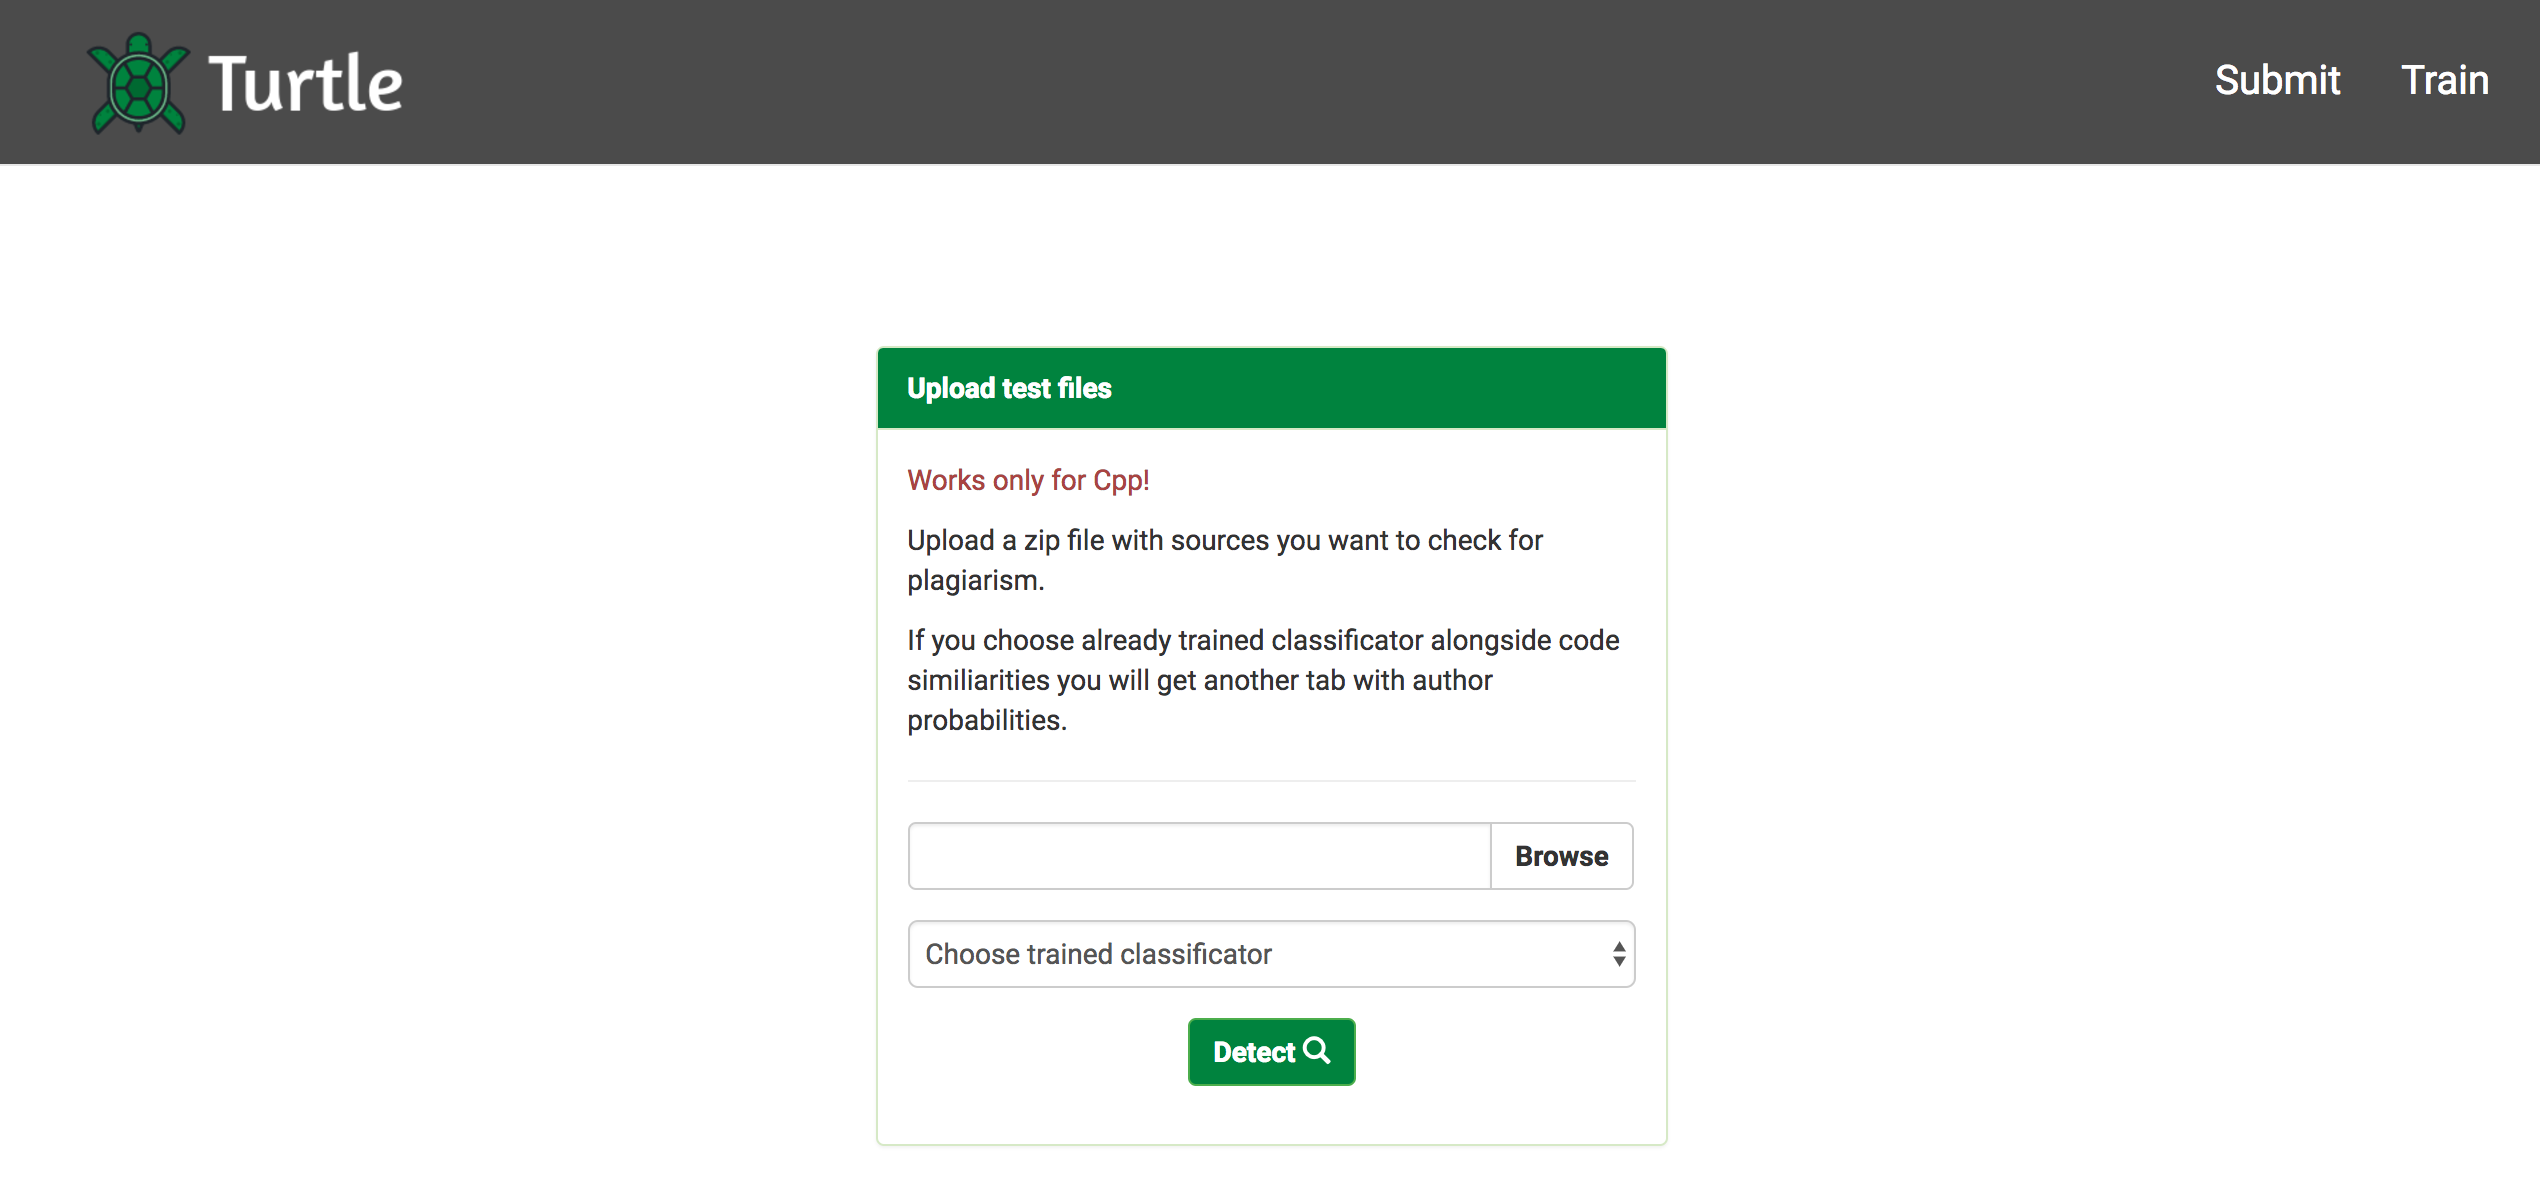
\includegraphics[width=0.8\textwidth,keepaspectratio]{fig/submit.png}
	\caption{Početna stranica, ovdje uploadamo zip datatoteku koju želimo provjeriti, također možemo izabrat unaprijed trenirani klasifikator kako bi mogli dobili i najvjerojatnije autore svakog koda.}
\end{figure}

\newpage
\vspace*{4cm}

\begin{figure}[htb]
	\centering
	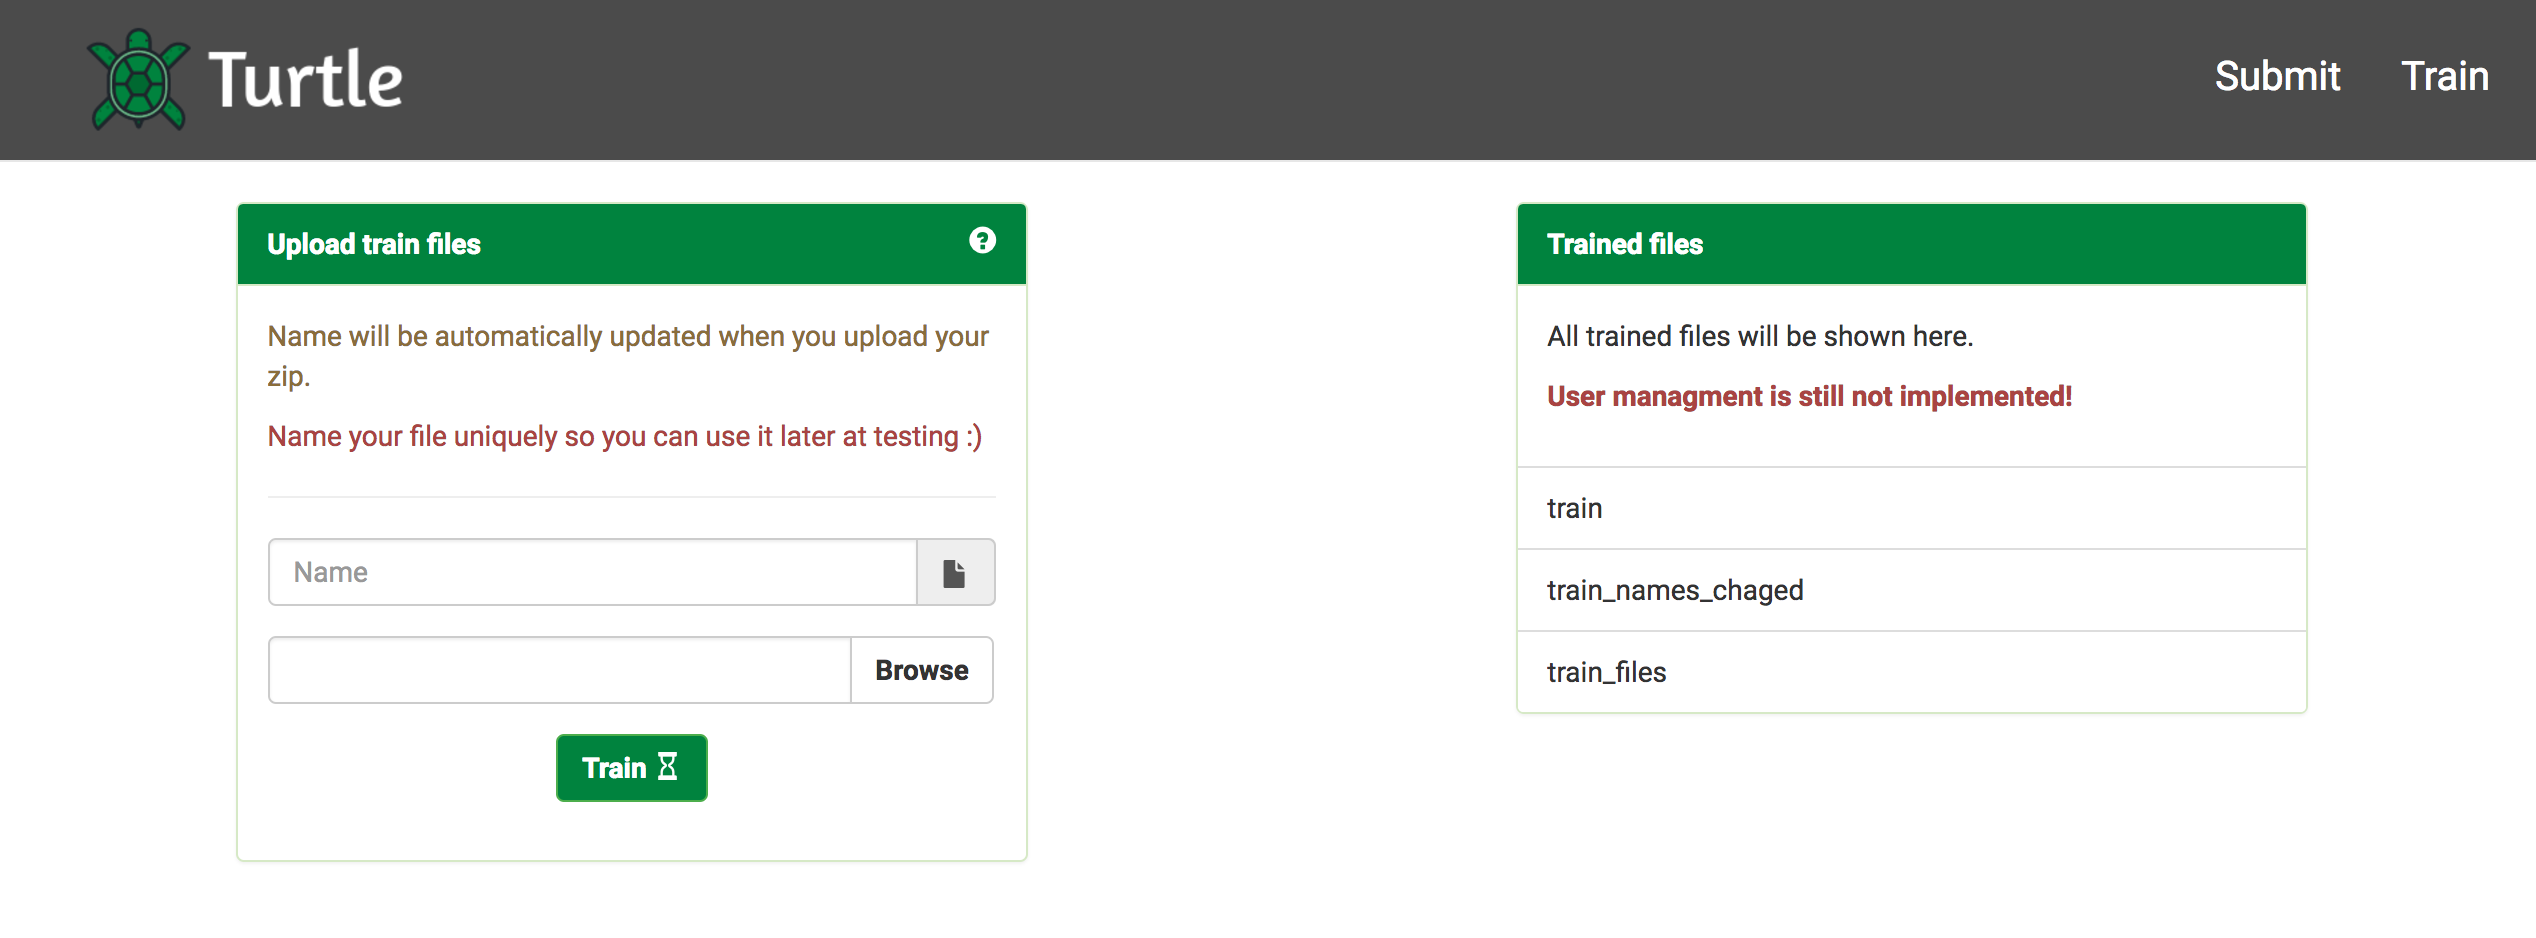
\includegraphics[width=0.8\textwidth,keepaspectratio]{fig/train.png}
	\caption{Stranica za treniranje klasifikatora, uploada se zip datoteka te nakon što je učenje završeno naučeni klasifikator se pojavi u listi desno.}
\end{figure}
\vspace*{4cm}
\begin{figure}[htb]
	\centering
	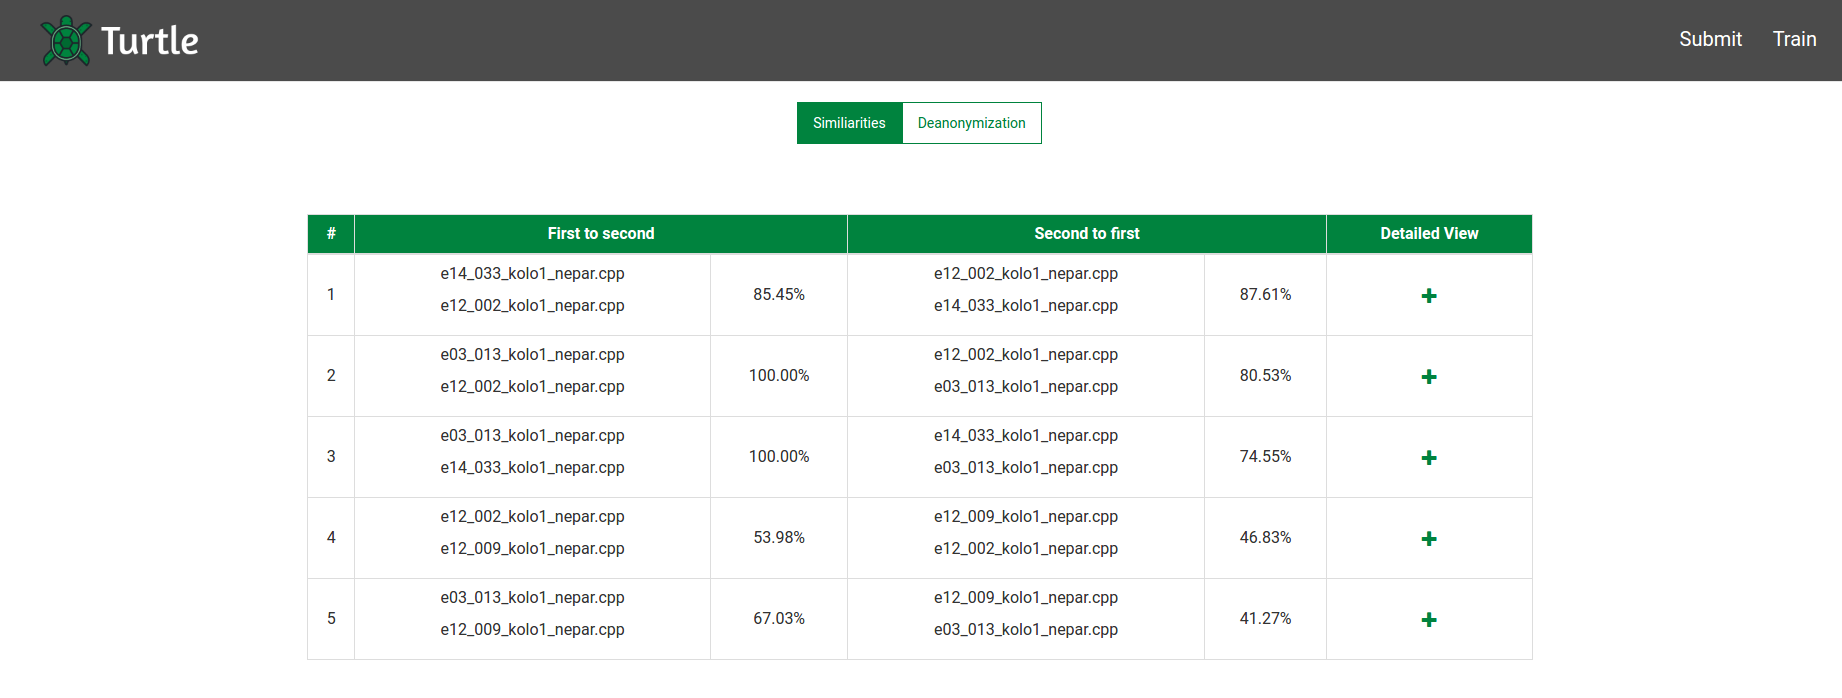
\includegraphics[width=0.8\textwidth,keepaspectratio]{fig/pairs.png}
	\caption{Nakon što sustav pronađe sve sličnosti ispiše nam ih u tablicu sortirane od najveće do najmanje sličnosti.}
\end{figure}

\newpage
\vspace*{2cm}
\begin{figure}[htb]
	\centering
	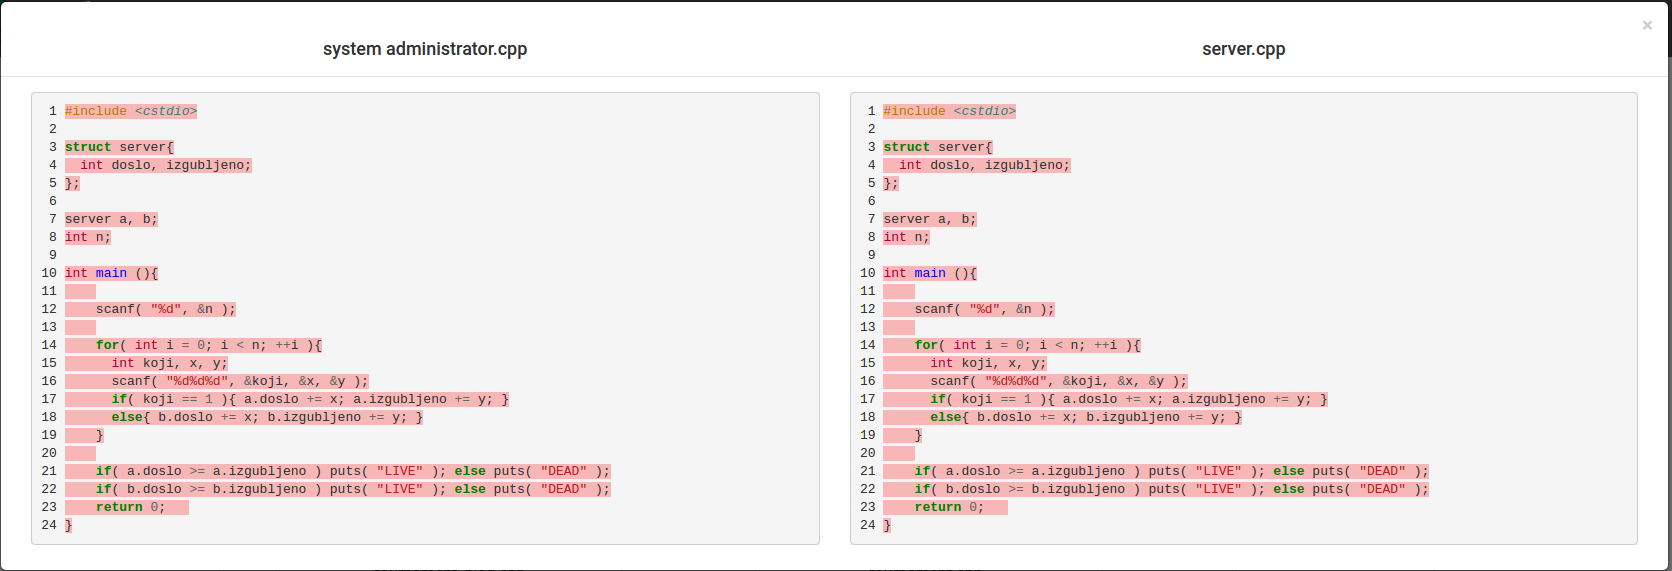
\includegraphics[width=0.8\textwidth,keepaspectratio]{fig/colors.png}
	\caption{Ako kliknemo na više detalja koji postoji za svaki par izvornih kodova dobijemo ovakav prozor gdje su obojani dijelovi koda koji su slični i što nam uvelike olakšava detekciju plagijata.}
\end{figure}
\vspace*{4cm}
\begin{figure}[htb]
	\centering
	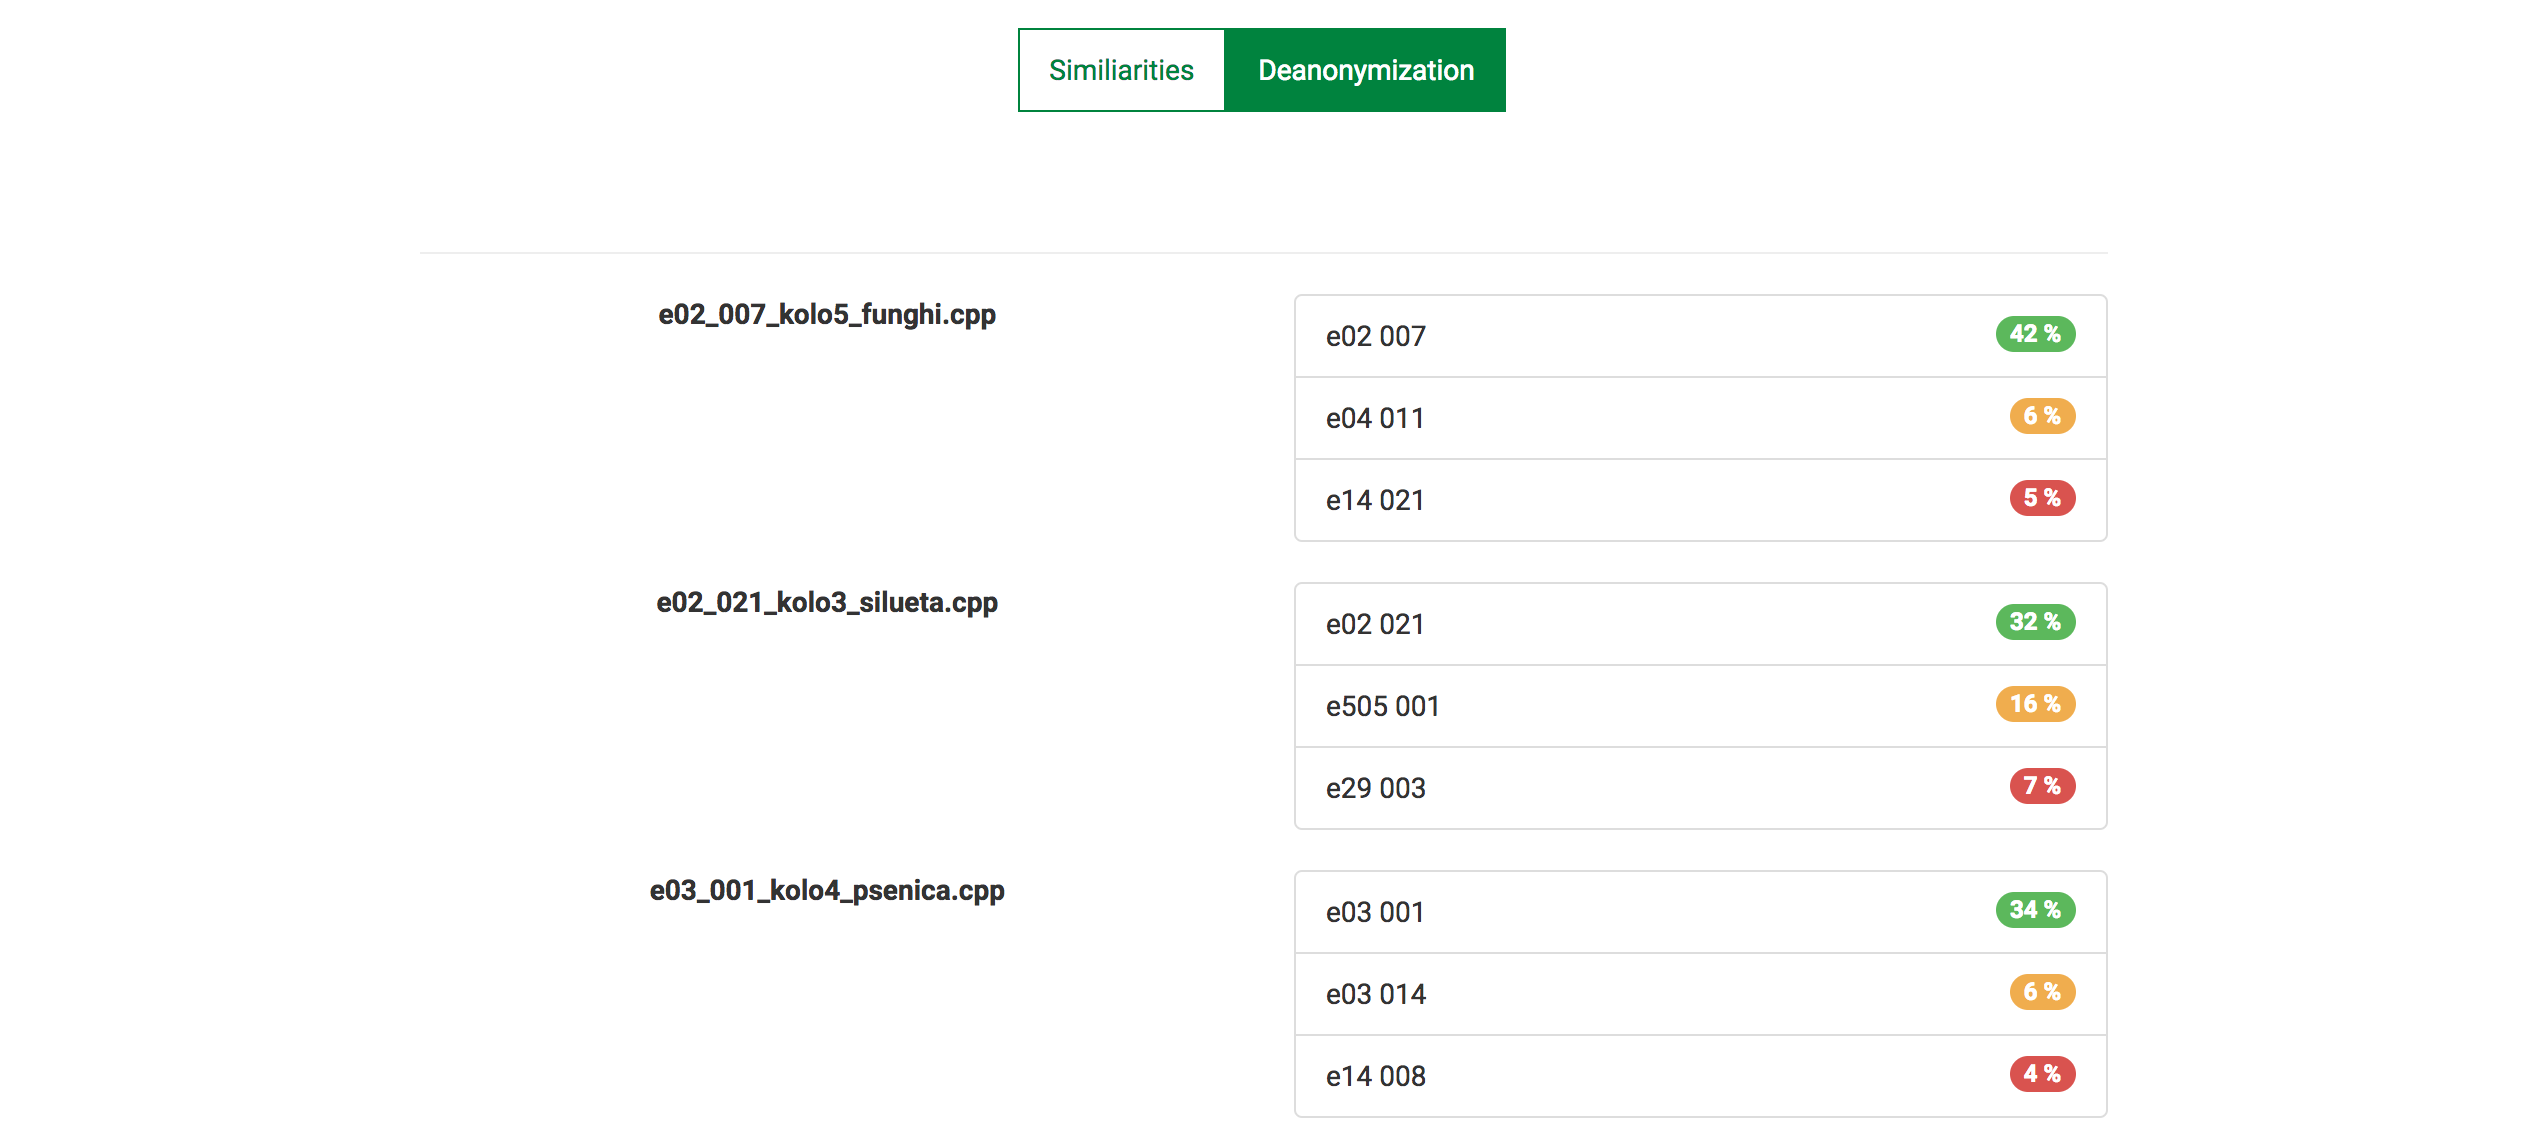
\includegraphics[width=0.8\textwidth,keepaspectratio]{fig/authors.png}
	\caption{Ako smo uz detekciju plagijata odredili da želimo i provjeriti tko bi mogli biti autori naših kodova na tabu \textit{Deanonymization} dobijemo za svaki izvorni kod listu od 3 najvjerojatnija autora.}
\end{figure}


\newpage

\section{Implementacijski detalji}

$Turtle$ je implementiran u $Python 2.7$ koristeći njegov framework $Flask$ \footnote{http://flask.pocoo.org/}. Klijentski dio aplikacije implementiran je u $ReactJS$ \footnote{https://facebook.github.io/react/} frameworku kako bi korisnici imali što bolji doživljan korištenja aplikacije te zbog asinkronog dohvata podataka.